% AA-62
\chapter[Prezentacja Serre'a]{Twierdzenie o prezentacji Serre'a}
\label{aa:ch:serre-presentation}

W poprzednim rozdziale wyprowadziliśmy relacje spełniane przez generatory istniejącej półprostej algebry Liego. Teraz zmieniamy kierunek rozumowania: punktem wyjścia jest skończony zredukowany krystalograficzny układ korzeni. Zbudujemy algebrę za pomocą samych generatorów i relacji, wykażemy jej skończony wymiar oraz półprostotę. W szczególności dowód istnienia nie będzie zakładał wcześniejszego istnienia algebry danego typu.

\section{Algebra zadana generatorami i relacjami}

Niech $K$ będzie ciałem algebraicznie domkniętym charakterystyki zero, $\Phi$ niepustym skończonym zredukowanym krystalograficznym układem korzeni w rzeczywistej przestrzeni euklidesowej $V$ oraz $\Delta=(\alpha_1,\ldots,\alpha_r)$ jego bazą. Przyjmujemy konwencję
\[
 a_{ij}=\frac{2(\alpha_i,\alpha_j)}{(\alpha_i,\alpha_i)}.
\]
Macierz $A=(a_{ij})$ jest odwracalna, gdyż po pomnożeniu z lewej przez diagonalną macierz o wyrazach $(\alpha_i,\alpha_i)/2$ otrzymujemy dodatnio określoną macierz Grama. Ponieważ $A$ ma współczynniki całkowite, jest odwracalna także nad $K$.

\begin{definicja}
\label{aa:def:serre-algebra}
Algebrą $\mathfrak s(A)$ nazywamy iloraz wolnej algebry Liego nad $K$ o generatorach $e_i,f_i,h_i$ ($1\le i\le r$) przez ideał generowany przez relacje
\[
\begin{aligned}
 [h_i,h_j]&=0,&[h_i,e_j]&=a_{ij}e_j,\\
 [h_i,f_j]&=-a_{ij}f_j,&[e_i,f_j]&=\delta_{ij}h_i
\end{aligned}
\]
oraz, dla $i\ne j$, przez
\[
 (\operatorname{ad}e_i)^{1-a_{ij}}e_j=0,\qquad
 (\operatorname{ad}f_i)^{1-a_{ij}}f_j=0.
\]
Przez te same symbole oznaczamy obrazy generatorów w ilorazie.
\end{definicja}

Wolną algebrę Liego można zbudować z przestrzeni liniowej formalnych słów nawiasowych przez iloraz wyznaczony przez antysymetrię i tożsamość Jacobiego. Każde przypisanie generatorom elementów innej algebry Liego przedłuża się do homomorfizmu dokładnie wtedy, gdy spełnia wszystkie zadane relacje. Na tym etapie nie wiemy nawet, czy obrazy $h_i$ są liniowo niezależne.

Oznaczmy przez $\mathfrak u^+$ i $\mathfrak u^-$ podalgebry generowane odpowiednio przez $e_i$ i $f_i$, a przez $H$ przestrzeń rozpiętą przez $h_i$. Niech $Q=\bigoplus_i\mathbb Z\alpha_i$ będzie kratą korzeniową. Nadajemy generatorom stopnie $\alpha_i,-\alpha_i,0$ odpowiednio dla $e_i,f_i,h_i$. Wszystkie relacje są jednorodne, więc iloraz ma gradację przez $Q$.

\begin{lemat}[Rozkład trójkątny przed dowodem istnienia]
\label{aa:lem:serre-triangular}
Dla algebry $\mathfrak s(A)$ z Definicji~\ref{aa:def:serre-algebra} zachodzi
\[
 \mathfrak s(A)=\mathfrak u^-\oplus H\oplus\mathfrak u^+.
\]
Przestrzeń stopnia zero jest równa $H$, a każdy niezerowy stopień ma współczynniki w bazie $\Delta$ albo wszystkie nieujemne, albo wszystkie niedodatnie.
\end{lemat}
\begin{proof}
Każda algebra Liego generowana przez zbiór $X$ jest rozpięta przez elementy $X$ oraz słowa postaci $[x_1,[x_2,\ldots,[x_{m-1},x_m]\ldots]]$, gdzie $x_i\in X$. Wynika to przez indukcję po długości pierwszego argumentu nawiasu, z tożsamości $[[x,y],z]=[x,[y,z]]-[y,[x,z]]$.

Dla każdego $i$ mamy $[e_i,\mathfrak u^-]\subset H+\mathfrak u^-$. Istotnie, dla słowa długości jeden jest to relacja $[e_i,f_j]=\delta_{ij}h_i$. Dla słowa $[f_j,w]$ stosujemy
\[
 [e_i,[f_j,w]]=[[e_i,f_j],w]+[f_j,[e_i,w]].
\]
Pierwszy składnik należy do $\mathfrak u^-$, ponieważ $[H,\mathfrak u^-]\subset\mathfrak u^-$ (co wynika indukcyjnie z relacji dla $h_i$). Drugi też należy do $\mathfrak u^-$ na mocy założenia indukcyjnego. Zamieniając $e_i$ z $f_i$ oraz $h_i$ z $-h_i$, otrzymujemy $[f_i,\mathfrak u^+]\subset H+\mathfrak u^+$.

Przestrzeń $T=\mathfrak u^-+H+\mathfrak u^+$ jest więc niezmiennicza względem nawiasu z każdym generatorem i zawiera wszystkie generatory. Z opisu słów nawiasowych wynika $T=\mathfrak s(A)$. Stopnie występujące w trzech składnikach są parami rozłączne: ujemne, zerowy oraz dodatnie. Suma jest zatem prosta.
\end{proof}

\section{Odbicia i ograniczenie wymiaru}

\begin{lemat}[Automorfizmy odpowiadające odbiciom]
\label{aa:lem:serre-reflections}
Niech $\mathfrak s(A)$ będzie algebrą z Definicji~\ref{aa:def:serre-algebra}. Operatory $\operatorname{ad}e_i$ i $\operatorname{ad}f_i$ są lokalnie nilpotentne: każdy element algebry jest zerowany przez pewną potęgę danego operatora. Automorfizm
\[
 R_i=\exp(\operatorname{ad}e_i)\,
      \exp(-\operatorname{ad}f_i)\,
      \exp(\operatorname{ad}e_i)
\]
przenosi składową stopnia $\beta\in Q$ na składową stopnia $s_i\beta$, gdzie $s_i$ jest odbiciem względem hiperpłaszczyzny prostopadłej do $\alpha_i$.
\end{lemat}
\begin{proof}
Lokalna nilpotentność na generatorach wynika z relacji: działanie na $h_j$ kończy się po dwóch krokach, na $f_i$ po trzech, na $f_j$ dla $j\ne i$ po jednym, a na $e_j$ dla $j\ne i$ z relacji Serre'a. Dla derywacji $D$ zachodzi wzór
\[
 D^m[x,y]=\sum_{k=0}^m\binom{m}{k}[D^kx,D^{m-k}y].
\]
Jeśli $D^p x=D^q y=0$, to $D^{p+q-1}[x,y]=0$. Indukcja po słowach nawiasowych i skończoność sum dowodzą tezy na całej algebrze; dla $f_i$ argument jest analogiczny. Szereg $\exp(D)x=\sum_{m\ge0}D^mx/m!$ jest zatem dla każdego $x$ skończony. Ten sam wzór dwumianowy daje $\exp(D)[x,y]=[\exp(D)x,\exp(D)y]$, zaś mnożenie skończonych szeregów na każdym elemencie daje odwrotność $\exp(-D)$.

Dla ustalonego $i$ bezpośrednio z relacji otrzymujemy
$\exp(\operatorname{ad}e_i)h_i=h_i-2e_i$,
$\exp(-\operatorname{ad}f_i)h_i=h_i-2f_i$ oraz
$\exp(-\operatorname{ad}f_i)e_i=e_i+h_i-f_i$.
Po złożeniu trzech odwzorowań wynika $R_i h_i=-h_i$. Element $h_j-(a_{ji}/2)h_i$ komutuje z $e_i,f_i$ i jest ustalony przez $R_i$. Zatem
\[
 R_i h_j=h_j-a_{ji}h_i,\qquad R_i^{-1}h_j=R_i h_j.
\]
Jeżeli $x$ ma stopień $\beta=\sum_k n_k\alpha_k$, to
$[h_j,x]=b_j x$, gdzie $b_j=\sum_k a_{jk}n_k$; wynika to indukcyjnie z relacji i tożsamości Jacobiego. W konsekwencji
\[
 [h_j,R_ix]=R_i[R_i^{-1}h_j,x]
 =(b_j-a_{ji}b_i)R_ix.
\]
Współrzędne $s_i\beta=\beta-b_i\alpha_i$ dają właśnie te wartości. Różne stopnie mają różne rodziny wartości własnych, ponieważ $A$ jest odwracalna nad $K$, a charakterystyka jest zero. Rozkładając $R_ix$ na skończenie wiele jednorodnych składowych, widzimy, że wszystkie poza stopniem $s_i\beta$ muszą znikać. Odwrotność $R_i^{-1}$ daje przeciwne zawieranie.
\end{proof}

\begin{twierdzenie}[Górne ograniczenie wymiaru]
\label{aa:tw:serre-upper-dimension}
Dla algebry z Definicji~\ref{aa:def:serre-algebra} niezerowe składowe o stopniu różnym od zera mogą wystąpić jedynie w stopniach należących do $\Phi$, a każda ma wymiar co najwyżej jeden. W szczególności
\[
 \dim_K\mathfrak s(A)\le r+|\Phi|.
\]
\end{twierdzenie}
\begin{proof}
Niech $\beta=\sum_i n_i\alpha_i$ będzie dodatnim stopniem o niezerowej składowej. Jeżeli jego nośnik składa się tylko z indeksu $i$, to wszystkie słowa tego stopnia są słowami w jednym generatorze $e_i$. Każde takie słowo długości większej niż jeden jest zerem, ponieważ $[e_i,e_i]=0$. Zatem jedyny możliwy stopień o jednoelementowym nośniku to $\alpha_i$, a jego składowa ma wymiar co najwyżej jeden.

Gdy nośnik ma co najmniej dwa elementy, z
$(\beta,\beta)=\sum_i n_i(\beta,\alpha_i)>0$
wynika istnienie $i$ z $n_i>0$ i $(\beta,\alpha_i)>0$. Liczba
$b_i=2(\beta,\alpha_i)/(\alpha_i,\alpha_i)$ jest dodatnią liczbą całkowitą. Stopień $s_i\beta=\beta-b_i\alpha_i$ ma niezerową składową na mocy Lematu~\ref{aa:lem:serre-reflections}. Współczynnik przy pewnym innym korzeniu prostym pozostaje dodatni. Z Lematu~\ref{aa:lem:serre-triangular} wszystkie współczynniki nowego stopnia są więc nieujemne. Jego wysokość zmniejszyła się o $b_i\ge1$.

Po skończonej liczbie takich kroków dochodzimy do stopnia prostego. Odbicia zachowują $\Phi$, więc wyjściowy stopień należy do $\Phi$, a jego składowa ma ten sam wymiar co składowa stopnia prostego. Ujemne stopnie badamy przez zamianę generatorów $e_i\leftrightarrow f_i$, $h_i\mapsto-h_i$, która zachowuje relacje i odwraca stopnie. Składowa zerowa ma wymiar co najwyżej $r$.
\end{proof}

\section{Konstrukcja modułów i niezależność generatorów}

Do wykazania dolnego ograniczenia wymiaru nie możemy użyć istnienia półprostej algebry Liego o zadanym układzie korzeni. Skonstruujemy moduły bezpośrednio z relacji.

\begin{twierdzenie}[Moduły z wektorem najwyższej wagi]
\label{aa:tw:serre-highest-module}
Niech $\mathfrak s(A)$ będzie algebrą z Definicji~\ref{aa:def:serre-algebra}. Dla każdej rodziny $\lambda=(\lambda_1,\ldots,\lambda_r)\in K^r$ istnieje jej moduł $M_\lambda$ z niezerowym wektorem $v_\lambda$ spełniającym
\[
 e_i v_\lambda=0,\quad h_i v_\lambda=\lambda_i v_\lambda,\quad
 f_i v_\lambda\ne0\qquad(1\le i\le r).
\]
\end{twierdzenie}
\begin{proof}
Niech $T=K\langle x_1,\ldots,x_r\rangle$ będzie wolną łączną algebrą z jedynką. Oznaczmy przez $F_i$ mnożenie z lewej przez $x_i$. Dla jednorodnego słowa $w$ z $n_j$ wystąpieniami $x_j$ definiujemy
\[
 H_iw=\left(\lambda_i-\sum_j a_{ij}n_j\right)w.
\]
Definiujemy liniowo operator $E_i$ rekurencją $E_i(1)=0$ oraz
\[
 E_i(x_jw)=x_jE_i(w)+\delta_{ij}H_iw.
\]
Każde niepuste słowo ma jednoznaczną pierwszą literę, więc rekurencja jest dobrze określona. Operator $E_i$ usuwa jedno wystąpienie $x_i$ (lub daje zero), co sprawdza się indukcyjnie. Wobec tego na $T$ zachodzą
\[
 [H_i,H_j]=0,\quad [H_i,F_j]=-a_{ij}F_j,\quad
 [H_i,E_j]=a_{ij}E_j,\quad [E_i,F_j]=\delta_{ij}H_i.
\]

Niech $J$ będzie dwustronnym ideałem $T$ generowanym przez
$S_{jk}=(\operatorname{ad}x_j)^{1-a_{jk}}x_k$ dla $j\ne k$, gdzie nawias w $T$ jest komutatorem. Jest to ideał jednorodny względem liczby wystąpień każdej litery, generowany w stopniach długości co najmniej dwa. Iloraz $T/J$ ma niezerową jedynkę oraz niezerowe obrazy wszystkich $x_i$.

Sprawdzimy, że $J$ jest niezmienniczy względem $E_i$. Oznaczmy $Y_m=(\operatorname{ad}F_j)^m F_k$ dla $j\ne k$. Wtedy $Y_m$ jest mnożeniem z lewej przez $(\operatorname{ad}x_j)^m x_k$. Mamy
$[H_j,Y_m]=(-a_{jk}-2m)Y_m$.
Dla $i=j$ indukcja daje
\[
 [E_j,Y_m]=m(-a_{jk}-m+1)Y_{m-1}\quad(m\ge1).
\]
Rzeczywiście dla $m=1$ otrzymujemy $[H_j,F_k]=-a_{jk}F_k$. W kroku indukcyjnym, z $Y_{m+1}=[F_j,Y_m]$, współczynnik wynosi
$-a_{jk}-2m+m(-a_{jk}-m+1)=(m+1)(-a_{jk}-m)$.
Dla $m=1-a_{jk}$ komutator znika. Jeśli $i$ jest różny od $j,k$, znika na mocy komutowania z $F_j,F_k$. Jeśli $i=k$, to $[E_k,Y_m]=(\operatorname{ad}F_j)^m H_k$. Dla $m\ge2$ wyrażenie jest zerem, ponieważ $[F_j,H_k]=a_{kj}F_j$. Gdy $m=1-a_{jk}=1$, mamy $a_{jk}=0$, a więc także $a_{kj}=0$. Ostatecznie $E_i$ komutuje z mnożeniem z lewej przez każdy $S_{jk}$.

Ideał $J$ jest rozpięty przez elementy $u S_{jk} w$ dla słów $u,w$. Jeżeli $u=1$, to
$E_i(S_{jk}w)=S_{jk}E_i(w)\in J$. Jeśli $u=x_lu'$, to rekurencja i niezmienniczość $J$ względem $H_i$ dają
\[
 E_i(x_lu'S_{jk}w)=x_l E_i(u'S_{jk}w)
                +\delta_{il}H_i(u'S_{jk}w)\in J.
\]
Zatem $E_i$, podobnie jak $H_i,F_i$, indukuje operator na $M_\lambda=T/J$.

Na ilorazie relacje Serre'a dla $F_i$ zachodzą z definicji $J$. Pozostają relacje dla $E_i$. Niech $Z=(\operatorname{ad}E_j)^{1-a_{jk}}E_k$. Ten sam rachunek komutatorów co wyżej, po zamianie $E_i$ z $F_i$ i $H_i$ z $-H_i$, daje $[F_i,Z]=0$ dla każdego $i$. Rachunek korzystał wyłącznie z czterech rodzin relacji liniowych, nie z relacji Serre'a. Ponadto $Z$ zeruje $1+J$, bo każdy iloczyn dodatniej liczby operatorów $E_i$ zeruje ten wektor. Wektory $F_{i_1}\cdots F_{i_l}(1+J)$ rozpinają $M_\lambda$. Komutowanie z $F_i$ pokazuje więc $Z=0$ na całym module. Wszystkie relacje z Definicji~\ref{aa:def:serre-algebra} są spełnione. Wystarczy przyjąć $v_\lambda=1+J$.
\end{proof}

\begin{wniosek}
\label{aa:cor:serre-dimension}
W algebrze $\mathfrak s(A)$ z Definicji~\ref{aa:def:serre-algebra} elementy $h_i$ są liniowo niezależne, wszystkie $e_i,f_i$ są niezerowe oraz
\[
 \dim_K\mathfrak s(A)=r+|\Phi|,
 \qquad \dim_K\mathfrak s(A)_\beta=1\quad(\beta\in\Phi).
\]
\end{wniosek}
\begin{proof}
Jeśli $\sum_i c_i h_i=0$, działanie na $v_\lambda$ daje $\sum_i c_i\lambda_i=0$ dla każdej $\lambda\in K^r$. Wybierając wektory jednostkowe, otrzymujemy $c_i=0$ dla każdego $i$. Elementy $f_i$ działają niezerowo na $v_\lambda$, a $e_i\ne0$ wynika z $[e_i,f_i]=h_i\ne0$. Każdy korzeń należy do orbity pewnego korzenia prostego względem grupy generowanej przez odbicia proste, na mocy Twierdzenia~\ref{aa:tw:weyl-chambers}. Stosując automorfizmy z Lematu~\ref{aa:lem:serre-reflections}, otrzymujemy niezerowe składowe dla wszystkich $\beta\in\Phi$. Twierdzenie~\ref{aa:tw:serre-upper-dimension} daje ich jednowymiarowość i wymaganą równość wymiarów.
\end{proof}

\section{Półprostota i twierdzenie o prezentacji}

\begin{twierdzenie}[Istnienie algebry o zadanym układzie korzeni]
\label{aa:tw:serre-existence}
Niech $K$ będzie algebraicznie domkniętym ciałem charakterystyki zero, $\Phi$ niepustym skończonym zredukowanym krystalograficznym układem korzeni, a $A$ macierzą Cartana jego bazy. Algebra $\mathfrak s(A)$ jest skończenie wymiarowa i półprosta. Podalgebra $H=\operatorname{span}_K\{h_1,\ldots,h_r\}$ jest maksymalną podalgebrą toralną, a układ korzeni względem $H$ odpowiada $\Phi$ przez przypisanie $\alpha_j(h_i)=a_{ij}$.
\end{twierdzenie}
\begin{proof}
Skończony wymiar wykazano w Twierdzeniu~\ref{aa:tw:serre-upper-dimension}. Z Wniosku~\ref{aa:cor:serre-dimension} elementy $h_i$ są liniowo niezależne. Działanie $\operatorname{ad}H$ jest diagonalne w rozkładzie na stopnie, a $H$ jest abelowa. Jeśli element komutuje z $H$, to wszystkie jego składowe o niezerowym stopniu muszą znikać, ponieważ macierz $A$ jest odwracalna. Centralizator $H$ jest więc równy $H$; żadna większa abelowa podalgebra nie może go zawierać. Korzenie w sensie rozkładu wagowego są dokładnie funkcjonałami odpowiadającymi stopniom $\beta\in\Phi$.

Niech $\mathfrak a$ będzie niezerowym rozwiązalnym ideałem $\mathfrak s(A)$. Wybierzmy $t\in H$ rozdzielający wszystkie wagi, łącznie z zerem. Istnieje on, ponieważ w przestrzeni $H$ nad nieskończonym ciałem skończona suma mnogościowa właściwych hiperpłaszczyzn nie pokrywa całej przestrzeni. Projekcje na składowe stopni są wielomianami w $\operatorname{ad}t$, jak w Lemacie~\ref{aa:lem:lie-ideal-weight-components}. Zatem ideał zawiera składowe każdego swojego elementu.

Jeśli zawiera niezerowy element składowej o stopniu $\beta\ne0$, to zawiera tę całą składową. Ideał jest niezmienniczy względem $\operatorname{ad}e_i,\operatorname{ad}f_i$, więc także względem ich skończonych wykładników i automorfizmów $R_i$ oraz odwrotnych. Możemy przenieść składową do stopnia prostego, otrzymując $e_i\in\mathfrak a$. Wówczas $[e_i,f_i]=h_i\in\mathfrak a$ i $[h_i,f_i]=-2f_i\in\mathfrak a$. Elementy $e_i,f_i,h_i$ rozpinają podalgebrę izomorficzną z $\mathfrak{sl}_2(K)$: relacje są standardowe, a niezależność wynika z różnych stopni i niezerowości. Jej algebra pochodna jest nią samą, co przeczy rozwiązalności $\mathfrak a$.

W przeciwnym przypadku $\mathfrak a\subset H$. Dla $0\ne t\in\mathfrak a$ odwracalność $A$ i niezależność $h_i$ dają indeks $j$ z $\alpha_j(t)\ne0$. Wtedy $[t,e_j]=\alpha_j(t)e_j\in\mathfrak a$, sprzeczność. Nie ma więc niezerowego rozwiązalnego ideału, czyli $\mathfrak s(A)$ jest półprosta.

Sprawdźmy jeszcze zgodność iloczynów skalarnych w realizacji korzeni. Dla pierwotnego układu $\Phi$ wartości $\beta(h_i)$ są liczbami całkowitymi wyznaczonymi przez $A$ i współrzędne $\beta$. Forma Killinga na $H$ jest zatem określona macierzą
$B_{ij}=\sum_{\beta\in\Phi}\beta(h_i)\beta(h_j)$.
W modelu rzeczywistym forma $B$ jest dodatnio określona, gdyż korzenie rozpinają przestrzeń. Jest niezmiennicza względem odbić, ponieważ odbicia permutują korzenie. W przestrzeni dualnej forma o macierzy $B^{-1}$ jest również niezmiennicza względem odbić. Odbicie $s_i$ ma kierunek zmiany $\alpha_i$ i hiperpłaszczyznę punktów stałych $\{\beta:\beta(h_i)=0\}$. Z ortogonalności względem tej formy otrzymujemy dla każdego $\beta$ stosunek Cartana równy $\beta(h_i)$. Realizacja euklidesowa z Twierdzenia~\ref{aa:tw:lie-root-realization} daje więc tę samą macierz Cartana $A$. Odwzorowanie liniowe przypisujące pierwotnym korzeniom prostym odpowiadające im wagi jest odwracalne, ponieważ $A$ jest odwracalna. Przenosi ono zbiór korzeni na zbiór wag niezerowych, jak już wykazaliśmy, i przeplata odbicia proste. Ponieważ każdy korzeń należy do orbity korzenia prostego, przeplata również odbicia odpowiadające wszystkim korzeniom, a tym samym zachowuje wszystkie liczby Cartana. Na każdej składowej nierozkładalnej można też zastosować Twierdzenie~\ref{aa:tw:root-uniqueness}: iloczyny skalarne różnią się jedynie dodatnim mnożnikiem, który może być różny dla różnych składowych.
\end{proof}

\begin{twierdzenie}[Prezentacja Serre'a]
\label{aa:tw:serre-presentation}
Niech $\mathfrak g$ będzie niezerową skończenie wymiarową półprostą algebrą Liego nad algebraicznie domkniętym ciałem $K$ charakterystyki zero, $\mathfrak h$ jej maksymalną podalgebrą toralną, $\Delta$ bazą układu korzeni, a $A$ odpowiadającą macierzą Cartana. Niech $e_i,f_i,h_i$ będą generatorami z Twierdzenia~\ref{aa:tw:lie-serre-necessary}. Istnieje dokładnie jeden izomorfizm $\mathfrak s(A)\to\mathfrak g$ przypisujący formalnym generatorom odpowiadające im elementy $\mathfrak g$.
\end{twierdzenie}
\begin{proof}
Relacje z AA-61 dają homomorfizm na mocy własności ilorazu wolnej algebry Liego. Jest on surjektywny, ponieważ obrazy $e_i,f_i$ generują $\mathfrak g$ (Twierdzenie~\ref{aa:tw:lie-simple-generators}). Rozkład korzeniowy w $\mathfrak g$ ma $r$ wymiarów w stopniu zero i po jednym wymiarze dla każdego korzenia. Stąd
$\dim\mathfrak g=r+|\Phi|=\dim\mathfrak s(A)$
na mocy Wniosku~\ref{aa:cor:serre-dimension}. Surjektywny homomorfizm jest zatem izomorfizmem. Jednoznaczność wynika z generowania.
\end{proof}

\section{Konsekwencje dla klasyfikacji}

\begin{wniosek}
\label{aa:cor:serre-classification-step}
Dla każdego niepustego skończonego zredukowanego krystalograficznego układu korzeni istnieje półprosta algebra Liego nad $K$ realizująca ten układ. Jeżeli dwie półproste algebry Liego nad $K$ mają, względem wybranych maksymalnych podalgebr toralnych i baz układów, tę samą macierz Cartana z dokładnością do jednoczesnej permutacji wierszy i kolumn, to są izomorficzne.
\end{wniosek}
\begin{proof}
Pierwsza teza wynika z Twierdzenia~\ref{aa:tw:serre-existence}. W drugiej po zmianie numeracji obie algebry są izomorficzne z tą samą $\mathfrak s(A)$ na mocy Twierdzenia~\ref{aa:tw:serre-presentation}.
\end{proof}

Dla nierozkładalnych układów z AA-56 uzyskujemy algebry proste, na mocy Twierdzenia~\ref{aa:tw:lie-dynkin-components}. Aby otrzymać pełną klasyfikację niezależną od wyboru maksymalnej podalgebry toralnej, pozostaje wykazać sprzężoność takich podalgebr. Nie używamy jej w niniejszym dowodzie i nie zakładamy, że została już udowodniona.

\begin{przyklad}
\label{aa:prz:serre-rank-two}
Dla macierzy $\left(\begin{smallmatrix}2&-3\\-1&2\end{smallmatrix}\right)$ typu $G_2$ niech $\alpha$ będzie krótszym, a $\beta$ dłuższym korzeniem prostym. Dodatnie korzenie to $\alpha,\beta,\alpha+\beta,2\alpha+\beta,3\alpha+\beta,3\alpha+2\beta$. Wniosek~\ref{aa:cor:serre-dimension} daje wymiar $2+12=14$. Relacje dodatnie to
\[
 (\operatorname{ad}e_1)^4e_2=0,\qquad
 (\operatorname{ad}e_2)^2e_1=0.
\]
W algebrze istniejącej na mocy Twierdzenia~\ref{aa:tw:serre-existence} poprzednie potęgi nie znikają, zgodnie z AA-61. Rozkład trójkątny ma wymiary $6+2+6$.
\end{przyklad}

\begin{center}
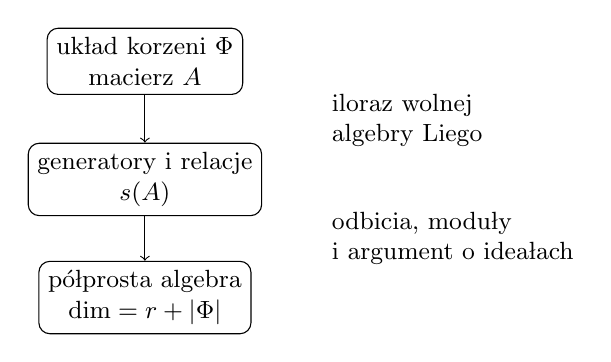
\begin{tikzpicture}[every node/.style={font=\small}]
\node[draw,rounded corners,align=center] (a) at (0,0) {układ korzeni $\Phi$\\macierz $A$};
\node[draw,rounded corners,align=center] (b) at (0,-1.5) {generatory i relacje\\$\mathfrak s(A)$};
\node[draw,rounded corners,align=center] (c) at (0,-3) {półprosta algebra\\$\dim=r+|\Phi|$};
\draw[->] (a)--(b);
\draw[->] (b)--(c);
\node[anchor=west,align=left] at (2.25,-.75) {iloraz wolnej\\algebry Liego};
\node[anchor=west,align=left] at (2.25,-2.25) {odbicia, moduły\\i argument o ideałach};
\end{tikzpicture}

\small Konstrukcja od układu korzeni do półprostej algebry Liego.
\end{center}
